\documentclass[12pt]{article}

\usepackage{sbc-template}
\usepackage{graphicx,url}
\usepackage[utf8]{inputenc}

%\usepackage[brazil]{babel}
%\usepackage[latin1]{inputenc}

\sloppy

\title{Relações Binárias em Conjuntos\\Trabalho Prático de Matemática Discreta}

\author{André Taiar\inst{1}}


\address{Departamento de Ciência da Computação -- Universidade Federal de Minas
Gerais (UFMG)\\
  \email{taiar@dcc.ufmg.br}
}

\begin{document}

\maketitle

\begin{resumo}
  Na matemática e na lógica, uma relação binária é uma relação qualquer entre
  dois elementos (um conjunto de pares ordenados). As relações binárias são comuns
  em muitas áreas da ciência para definir muitas propriedades e conceitos. Neste
  trabalho, foram analisados arquivos que mapeavam diversos conjuntos e as
  relações entre seus elementos e essas foram classificadas de acordo com as
  suas propriedades.
\end{resumo}


\section{Relações em grafos} %mudar esse título

Em matemática e ciência da computação, grafo é o objeto básico de estudo da
teoria dos grafos. Tipicamente, um grafo é representado como um conjunto de
pontos (vértices) ligados por retas (as arestas).

\begin{figure}[ht]
\centering

\includegraphics[width=.5\textwidth]{grafoEx.png}
\caption{Exemplo ilustrativo de um grafo com 6 vértices e 7 arestas}
\label{fig:exampleFig1}
\end{figure}

Utilizei neste trabalho um grafo para representar a relação entre os elementos
que foram passados na entrada. Cada elemento é representado como um vértice do
grafo e, se um elemento tem relação com outro elemento qualquer, eles são ligados
por uma aresta.

Para facilitar a análise das relações através do grafo, este foi implementado
utilizando uma matriz de adjacência como veremos no detalhamento das estruturas de
dados.

\section{Estruturas de dados e implementações}

O programa foi desenvolvido em 4 módulos: o módulo principal que cuida da leitura
do arquivo de entrada, da geração da saída e da lógica do funcionamento do programa
em si, o módulo que contém a implementação do grafo por matriz de adjacência, um
módulo com a implementação de uma lista encadeada utilizada em diversas partes
do programa e um módulo com a implementação da análise das relações utilizando o grafo.

\subsection{Implementação do grafo}

\subsection{Lista encadeada}

\subsection{Análise das relações}

\section{CD-ROMs and Printed Proceedings}

In some conferences, the papers are published on CD-ROM while only the
abstract is published in the printed Proceedings. In this case, authors are
invited to prepare two final versions of the paper. One, complete, to be
published on the CD and the other, containing only the first page, with
abstract and ``resumo'' (for papers in Portuguese).

\section{Sections and Paragraphs}

Section titles must be in boldface, 13pt, flush left. There should be an extra
12 pt of space before each title. Section numbering is optional. The first
paragraph of each section should not be indented, while the first lines of
subsequent paragraphs should be indented by 1.27 cm.

\subsection{Subsections}

The subsection titles must be in boldface, 12pt, flush left.

\section{Figures and Captions}\label{sec:figs}


Figure and table captions should be centered if less than one line
(Figure~\ref{fig:exampleFig1}), otherwise justified and indented by 0.8cm on
both margins, as shown in Figure~\ref{fig:exampleFig2}. The caption font must
be Helvetica, 10 point, boldface, with 6 points of space before and after each
caption.

\begin{figure}[ht]
\centering
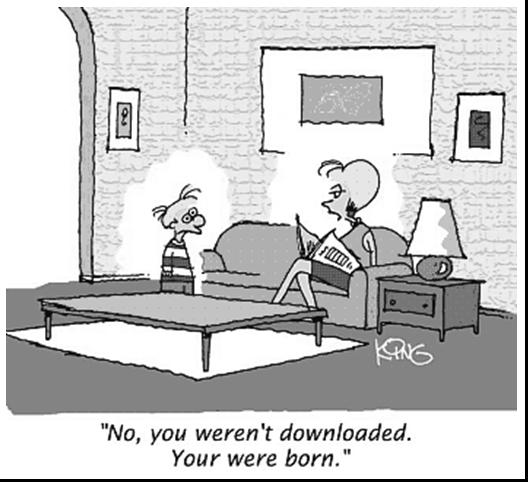
\includegraphics[width=.5\textwidth]{fig1.jpg}
\caption{A typical figure}
\label{fig:exampleFig1}
\end{figure}

\begin{figure}[ht]
\centering
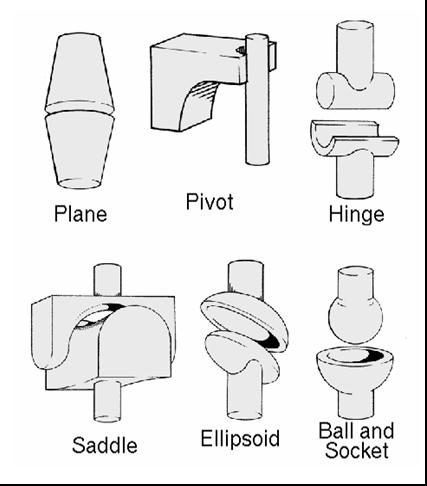
\includegraphics[width=.3\textwidth]{fig2.jpg}
\caption{This figure is an example of a figure caption taking more than one
  line and justified considering margins mentioned in Section~\ref{sec:figs}.}
\label{fig:exampleFig2}
\end{figure}

In tables, try to avoid the use of colored or shaded backgrounds, and avoid
thick, doubled, or unnecessary framing lines. When reporting empirical data,
do not use more decimal digits than warranted by their precision and
reproducibility. Table caption must be placed before the table (see Table 1)
and the font used must also be Helvetica, 10 point, boldface, with 6 points of
space before and after each caption.

\begin{table}[ht]
\centering
\caption{Variables to be considered on the evaluation of interaction
  techniques}
\label{tab:exTable1}
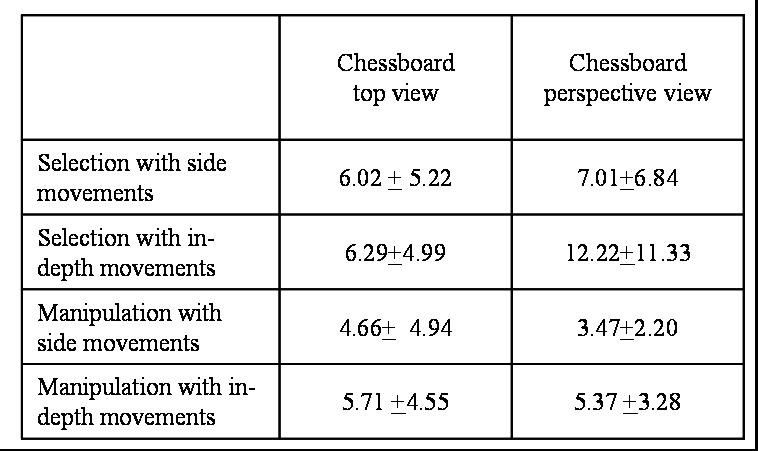
\includegraphics[width=.7\textwidth]{table.jpg}
\end{table}

\section{Images}

All images and illustrations should be in black-and-white, or gray tones,
excepting for the papers that will be electronically available (on CD-ROMs,
internet, etc.). The image resolution on paper should be about 600 dpi for
black-and-white images, and 150-300 dpi for grayscale images.  Do not include
images with excessive resolution, as they may take hours to print, without any
visible difference in the result.

\section{References}

Bibliographic references must be unambiguous and uniform.  We recommend giving
the author names references in brackets, e.g. \cite{knuth:84},
\cite{boulic:91}, and \cite{smith:99}.

The references must be listed using 12 point font size, with 6 points of space
before each reference. The first line of each reference should not be
indented, while the subsequent should be indented by 0.5 cm.

\bibliographystyle{sbc}
\bibliography{sbc-template}

\end{document}
